\documentclass{standalone}
\usepackage{tikz}
\usetikzlibrary{patterns, positioning}
\usepackage[sfdefault]{ClearSans} %% option 'sfdefault' activates Clear Sans as the default text font
\usepackage[T1]{fontenc}

\begin{document}
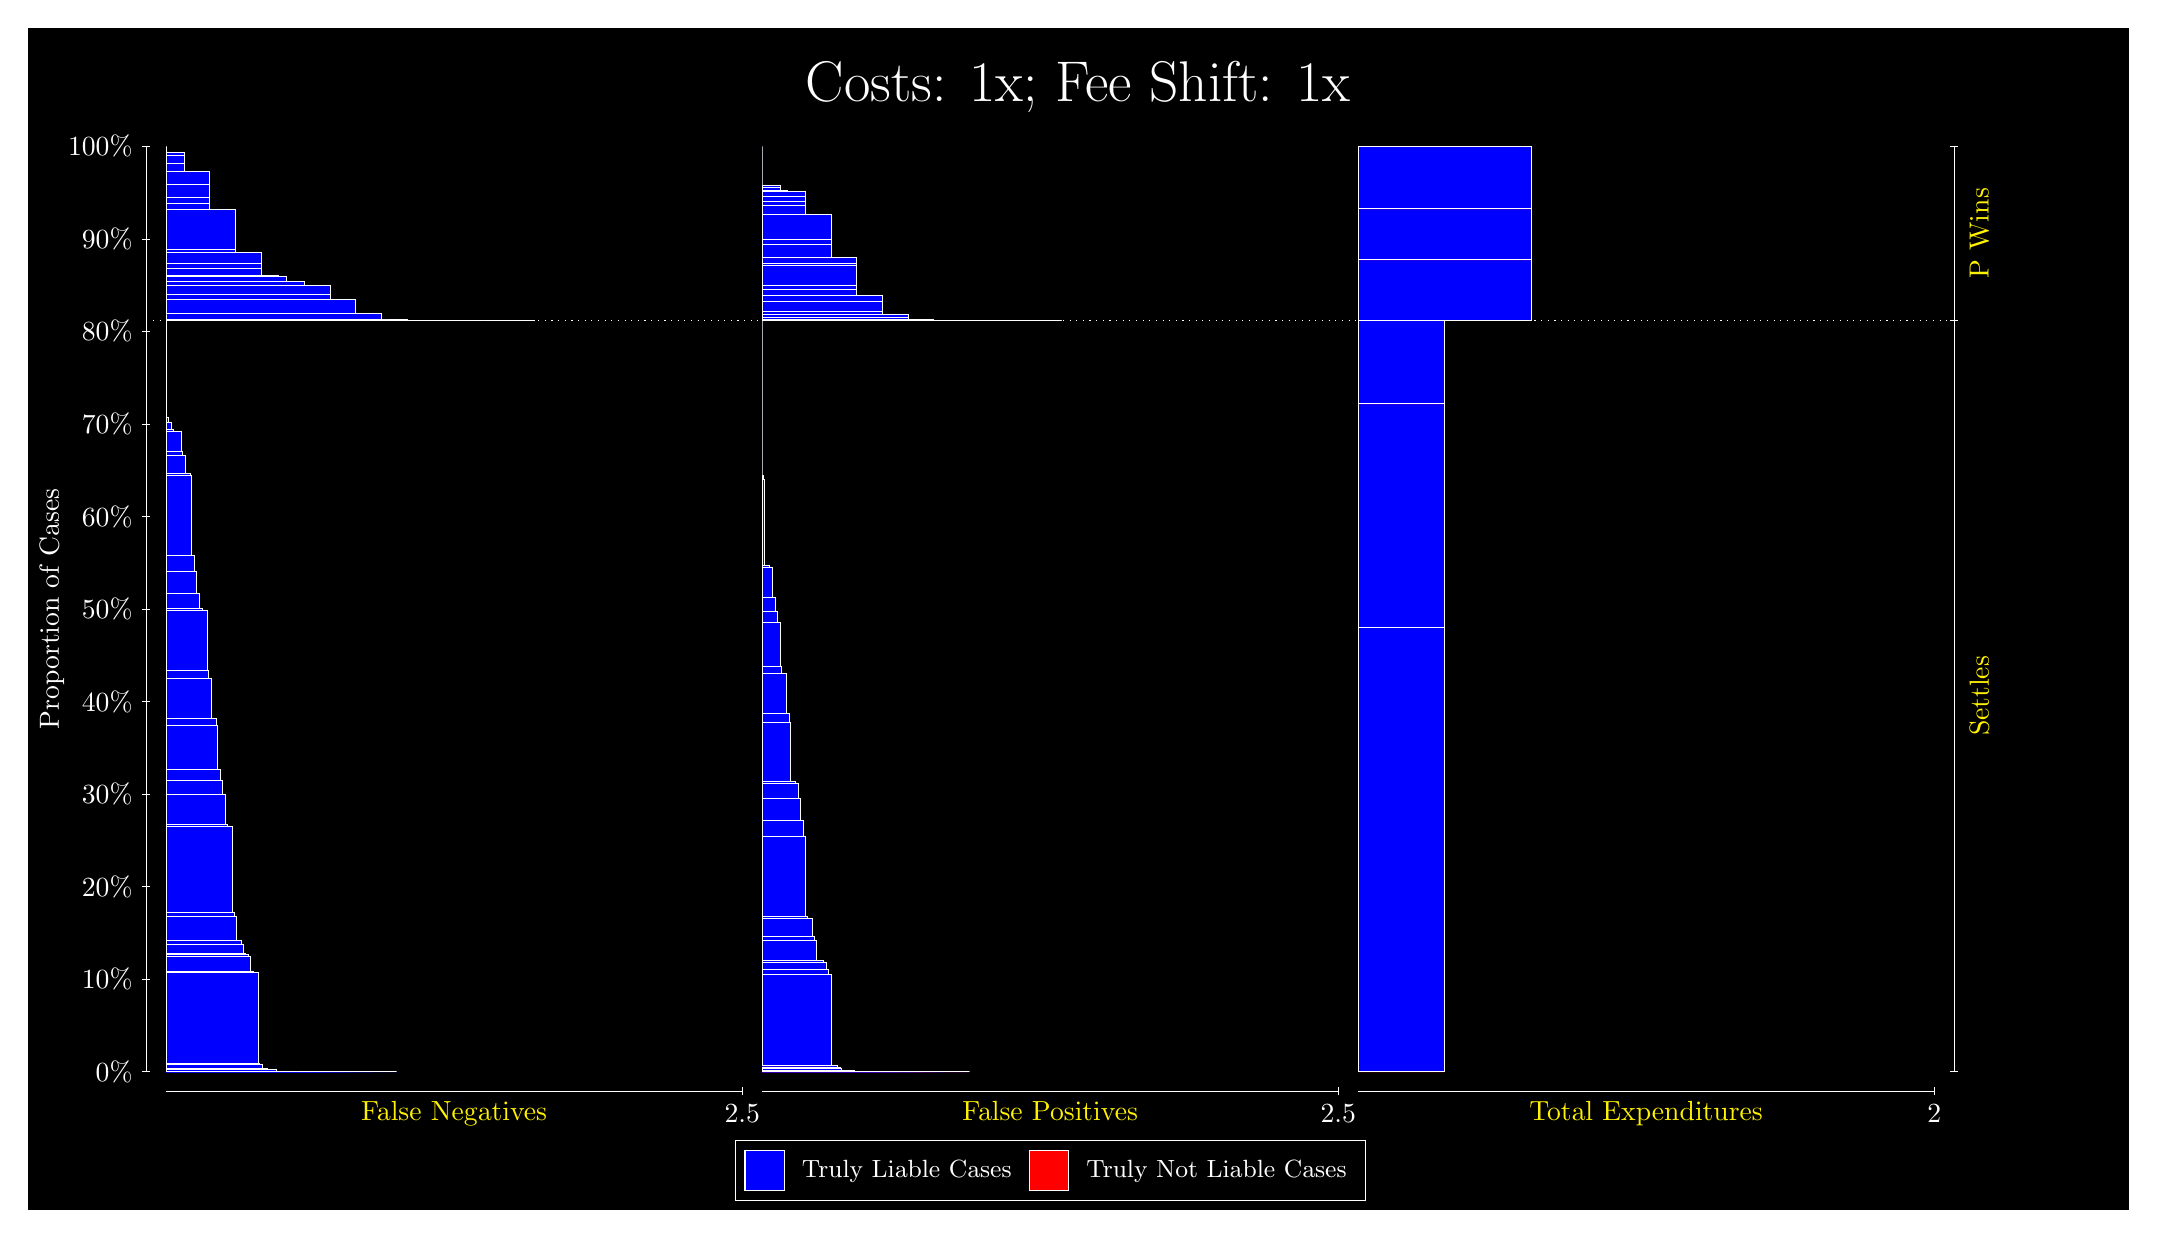
\begin{tikzpicture}
\draw[fill=black] (0,0) rectangle (26.667,15);
\draw[text=white] (0,13.5) rectangle (26.667,15) node[midway] {\huge Costs: 1x; Fee Shift: 1x};
\draw[white, very thin] (1.5,1.75) -- (1.5,13.5);
\node[rotate=90, text=white, anchor=center] at (0.3, 7.625) {Proportion of Cases};
\draw[white, very thin] (1.45,1.75) -- (1.55,1.75);
\node[text=white, anchor=east] at (1.45, 1.75) {0\%};
\draw[white, very thin] (1.45,2.925) -- (1.55,2.925);
\node[text=white, anchor=east] at (1.45, 2.925) {10\%};
\draw[white, very thin] (1.45,4.1) -- (1.55,4.1);
\node[text=white, anchor=east] at (1.45, 4.1) {20\%};
\draw[white, very thin] (1.45,5.275) -- (1.55,5.275);
\node[text=white, anchor=east] at (1.45, 5.275) {30\%};
\draw[white, very thin] (1.45,6.45) -- (1.55,6.45);
\node[text=white, anchor=east] at (1.45, 6.45) {40\%};
\draw[white, very thin] (1.45,7.625) -- (1.55,7.625);
\node[text=white, anchor=east] at (1.45, 7.625) {50\%};
\draw[white, very thin] (1.45,8.8) -- (1.55,8.8);
\node[text=white, anchor=east] at (1.45, 8.8) {60\%};
\draw[white, very thin] (1.45,9.975) -- (1.55,9.975);
\node[text=white, anchor=east] at (1.45, 9.975) {70\%};
\draw[white, very thin] (1.45,11.15) -- (1.55,11.15);
\node[text=white, anchor=east] at (1.45, 11.15) {80\%};
\draw[white, very thin] (1.45,12.325) -- (1.55,12.325);
\node[text=white, anchor=east] at (1.45, 12.325) {90\%};
\draw[white, very thin] (1.45,13.5) -- (1.55,13.5);
\node[text=white, anchor=east] at (1.45, 13.5) {100\%};

\draw[white, very thin] (24.457,1.75) -- (24.457,13.5);
\draw[white, very thin] (24.407,1.75) -- (24.507,1.75);
\node[anchor=west] at (24.407, 1.75) {};
\draw[white, very thin] (24.407,11.292) -- (24.507,11.292);
\node[anchor=west] at (24.407, 11.292) {};
\draw[white, very thin] (24.407,13.5) -- (24.507,13.5);
\node[anchor=west] at (24.407, 13.5) {};

\draw[white, very thin, fill=blue] (1.75,1.75) rectangle (4.6775,1.75);
\draw[white, very thin, fill=blue] (1.75,1.75) rectangle (4.3848,1.75);
\draw[white, very thin, fill=blue] (1.75,1.75) rectangle (4.3523,1.75);
\draw[white, very thin, fill=blue] (1.75,1.75) rectangle (4.2384,1.75);
\draw[white, very thin, fill=blue] (1.75,1.75) rectangle (4.092,1.75);
\draw[white, very thin, fill=blue] (1.75,1.75) rectangle (4.0595,1.75);
\draw[white, very thin, fill=blue] (1.75,1.75) rectangle (4.027,1.75);
\draw[white, very thin, fill=blue] (1.75,1.75) rectangle (3.9457,1.75);
\draw[white, very thin, fill=blue] (1.75,1.75) rectangle (3.9131,1.75);
\draw[white, very thin, fill=blue] (1.75,1.75) rectangle (3.7993,1.75);
\draw[white, very thin, fill=blue] (1.75,1.75) rectangle (3.7668,1.75);
\draw[white, very thin, fill=blue] (1.75,1.75) rectangle (3.7342,1.75);
\draw[white, very thin, fill=blue] (1.75,1.75) rectangle (3.7017,1.75);
\draw[white, very thin, fill=blue] (1.75,1.75) rectangle (3.6204,1.75);
\draw[white, very thin, fill=blue] (1.75,1.75) rectangle (3.5878,1.75);
\draw[white, very thin, fill=blue] (1.75,1.75) rectangle (3.5065,1.75);
\draw[white, very thin, fill=blue] (1.75,1.75) rectangle (3.474,1.7506);
\draw[white, very thin, fill=blue] (1.75,1.7506) rectangle (3.4415,1.7506);
\draw[white, very thin, fill=blue] (1.75,1.7506) rectangle (3.4089,1.7506);
\draw[white, very thin, fill=blue] (1.75,1.7506) rectangle (3.3764,1.7506);
\draw[white, very thin, fill=blue] (1.75,1.7506) rectangle (3.3602,1.751);
\draw[white, very thin, fill=blue] (1.75,1.751) rectangle (3.2951,1.7533);
\draw[white, very thin, fill=blue] (1.75,1.7533) rectangle (3.2626,1.7535);
\draw[white, very thin, fill=blue] (1.75,1.7535) rectangle (3.1812,1.7537);
\draw[white, very thin, fill=blue] (1.75,1.7537) rectangle (3.1487,1.776);
\draw[white, very thin, fill=blue] (1.75,1.776) rectangle (3.1162,1.7764);
\draw[white, very thin, fill=blue] (1.75,1.7764) rectangle (3.0837,1.7769);
\draw[white, very thin, fill=blue] (1.75,1.7769) rectangle (3.0511,1.7821);
\draw[white, very thin, fill=blue] (1.75,1.7821) rectangle (3.0349,1.7891);
\draw[white, very thin, fill=blue] (1.75,1.7891) rectangle (2.9698,1.8427);
\draw[white, very thin, fill=blue] (1.75,1.8427) rectangle (2.9373,1.8491);
\draw[white, very thin, fill=blue] (1.75,1.8491) rectangle (2.921,3.0131);
\draw[white, very thin, fill=blue] (1.75,3.0131) rectangle (2.856,3.0182);
\draw[white, very thin, fill=blue] (1.75,3.0182) rectangle (2.8234,3.213);
\draw[white, very thin, fill=blue] (1.75,3.213) rectangle (2.7909,3.2345);
\draw[white, very thin, fill=blue] (1.75,3.2345) rectangle (2.7584,3.2535);
\draw[white, very thin, fill=blue] (1.75,3.2535) rectangle (2.7258,3.3652);
\draw[white, very thin, fill=blue] (1.75,3.3652) rectangle (2.7096,3.4146);
\draw[white, very thin, fill=blue] (1.75,3.4146) rectangle (2.6445,3.7224);
\draw[white, very thin, fill=blue] (1.75,3.7224) rectangle (2.612,3.7762);
\draw[white, very thin, fill=blue] (1.75,3.7762) rectangle (2.5957,4.8598);
\draw[white, very thin, fill=blue] (1.75,4.8598) rectangle (2.5307,4.884);
\draw[white, very thin, fill=blue] (1.75,4.884) rectangle (2.4982,5.2743);
\draw[white, very thin, fill=blue] (1.75,5.2743) rectangle (2.4656,5.4517);
\draw[white, very thin, fill=blue] (1.75,5.4517) rectangle (2.4331,5.5905);
\draw[white, very thin, fill=blue] (1.75,5.5905) rectangle (2.4006,6.1491);
\draw[white, very thin, fill=blue] (1.75,6.1491) rectangle (2.3843,6.2368);
\draw[white, very thin, fill=blue] (1.75,6.2368) rectangle (2.3192,6.7397);
\draw[white, very thin, fill=blue] (1.75,6.7397) rectangle (2.2867,6.8514);
\draw[white, very thin, fill=blue] (1.75,6.8514) rectangle (2.2705,7.6072);
\draw[white, very thin, fill=blue] (1.75,7.6072) rectangle (2.2054,7.6309);
\draw[white, very thin, fill=blue] (1.75,7.6309) rectangle (2.1729,7.826);
\draw[white, very thin, fill=blue] (1.75,7.826) rectangle (2.1403,8.1072);
\draw[white, very thin, fill=blue] (1.75,8.1072) rectangle (2.1078,8.3043);
\draw[white, very thin, fill=blue] (1.75,8.3043) rectangle (2.0753,9.3171);
\draw[white, very thin, fill=blue] (1.75,9.3171) rectangle (2.059,9.3472);
\draw[white, very thin, fill=blue] (1.75,9.3472) rectangle (1.994,9.5735);
\draw[white, very thin, fill=blue] (1.75,9.5735) rectangle (1.9614,9.628);
\draw[white, very thin, fill=blue] (1.75,9.628) rectangle (1.9452,9.8785);
\draw[white, very thin, fill=blue] (1.75,9.8785) rectangle (1.8801,9.8831);
\draw[white, very thin, fill=blue] (1.75,9.8831) rectangle (1.8476,9.9051);
\draw[white, very thin, fill=blue] (1.75,9.9051) rectangle (1.8151,9.9921);
\draw[white, very thin, fill=blue] (1.75,9.9921) rectangle (1.7825,10.063);
\draw[white, very thin, fill=red] (1.75,10.063) rectangle (1.75,10.063);
\draw[white, very thin, fill=blue] (1.75,10.063) rectangle (1.75,11.292);
\draw[white, very thin, fill=blue] (1.75,11.292) rectangle (6.4341,11.292);
\draw[white, very thin, fill=blue] (1.75,11.292) rectangle (6.1088,11.292);
\draw[white, very thin, fill=blue] (1.75,11.292) rectangle (5.7835,11.292);
\draw[white, very thin, fill=blue] (1.75,11.292) rectangle (5.4582,11.292);
\draw[white, very thin, fill=blue] (1.75,11.292) rectangle (5.1329,11.294);
\draw[white, very thin, fill=blue] (1.75,11.294) rectangle (4.9052,11.294);
\draw[white, very thin, fill=blue] (1.75,11.294) rectangle (4.8077,11.3);
\draw[white, very thin, fill=blue] (1.75,11.3) rectangle (4.8077,11.307);
\draw[white, very thin, fill=blue] (1.75,11.307) rectangle (4.58,11.307);
\draw[white, very thin, fill=blue] (1.75,11.307) rectangle (4.58,11.307);
\draw[white, very thin, fill=blue] (1.75,11.307) rectangle (4.4824,11.375);
\draw[white, very thin, fill=blue] (1.75,11.375) rectangle (4.2547,11.375);
\draw[white, very thin, fill=blue] (1.75,11.375) rectangle (4.2547,11.375);
\draw[white, very thin, fill=blue] (1.75,11.375) rectangle (4.1571,11.555);
\draw[white, very thin, fill=blue] (1.75,11.555) rectangle (3.9294,11.555);
\draw[white, very thin, fill=blue] (1.75,11.555) rectangle (3.8318,11.621);
\draw[white, very thin, fill=blue] (1.75,11.621) rectangle (3.8318,11.734);
\draw[white, very thin, fill=blue] (1.75,11.734) rectangle (3.6041,11.738);
\draw[white, very thin, fill=blue] (1.75,11.738) rectangle (3.5065,11.79);
\draw[white, very thin, fill=blue] (1.75,11.79) rectangle (3.2788,11.791);
\draw[white, very thin, fill=blue] (1.75,11.791) rectangle (3.2788,11.852);
\draw[white, very thin, fill=blue] (1.75,11.852) rectangle (3.1812,11.857);
\draw[white, very thin, fill=blue] (1.75,11.857) rectangle (2.9535,11.86);
\draw[white, very thin, fill=blue] (1.75,11.86) rectangle (2.9535,11.947);
\draw[white, very thin, fill=blue] (1.75,11.947) rectangle (2.9535,12.016);
\draw[white, very thin, fill=blue] (1.75,12.016) rectangle (2.9535,12.157);
\draw[white, very thin, fill=blue] (1.75,12.157) rectangle (2.856,12.157);
\draw[white, very thin, fill=blue] (1.75,12.157) rectangle (2.6283,12.188);
\draw[white, very thin, fill=blue] (1.75,12.188) rectangle (2.6283,12.704);
\draw[white, very thin, fill=blue] (1.75,12.704) rectangle (2.5307,12.704);
\draw[white, very thin, fill=blue] (1.75,12.704) rectangle (2.303,12.779);
\draw[white, very thin, fill=blue] (1.75,12.779) rectangle (2.303,12.857);
\draw[white, very thin, fill=blue] (1.75,12.857) rectangle (2.303,13.013);
\draw[white, very thin, fill=blue] (1.75,13.013) rectangle (2.303,13.178);
\draw[white, very thin, fill=blue] (1.75,13.178) rectangle (2.2054,13.178);
\draw[white, very thin, fill=blue] (1.75,13.178) rectangle (1.9777,13.281);
\draw[white, very thin, fill=blue] (1.75,13.281) rectangle (1.9777,13.388);
\draw[white, very thin, fill=blue] (1.75,13.388) rectangle (1.9777,13.419);
\draw[white, very thin, fill=red] (1.75,13.419) rectangle (1.75,13.419);
\draw[white, very thin, fill=blue] (1.75,13.419) rectangle (1.75,13.5);
\draw[white, very thin, fill=red] (9.3189,1.75) rectangle (11.954,1.75);
\draw[white, very thin, fill=blue] (9.3189,1.75) rectangle (11.954,1.75);
\draw[white, very thin, fill=blue] (9.3189,1.75) rectangle (11.628,1.75);
\draw[white, very thin, fill=red] (9.3189,1.75) rectangle (11.515,1.75);
\draw[white, very thin, fill=blue] (9.3189,1.75) rectangle (11.515,1.75);
\draw[white, very thin, fill=red] (9.3189,1.75) rectangle (11.368,1.75);
\draw[white, very thin, fill=blue] (9.3189,1.75) rectangle (11.368,1.75);
\draw[white, very thin, fill=blue] (9.3189,1.75) rectangle (11.303,1.75);
\draw[white, very thin, fill=blue] (9.3189,1.75) rectangle (11.189,1.75);
\draw[white, very thin, fill=red] (9.3189,1.75) rectangle (11.075,1.75);
\draw[white, very thin, fill=blue] (9.3189,1.75) rectangle (11.075,1.75);
\draw[white, very thin, fill=blue] (9.3189,1.75) rectangle (11.043,1.75);
\draw[white, very thin, fill=blue] (9.3189,1.75) rectangle (10.978,1.75);
\draw[white, very thin, fill=red] (9.3189,1.75) rectangle (10.929,1.75);
\draw[white, very thin, fill=blue] (9.3189,1.75) rectangle (10.929,1.75);
\draw[white, very thin, fill=blue] (9.3189,1.75) rectangle (10.864,1.75);
\draw[white, very thin, fill=red] (9.3189,1.75) rectangle (10.783,1.75);
\draw[white, very thin, fill=blue] (9.3189,1.75) rectangle (10.783,1.7501);
\draw[white, very thin, fill=blue] (9.3189,1.7501) rectangle (10.75,1.7501);
\draw[white, very thin, fill=blue] (9.3189,1.7501) rectangle (10.718,1.7501);
\draw[white, very thin, fill=blue] (9.3189,1.7501) rectangle (10.653,1.7506);
\draw[white, very thin, fill=red] (9.3189,1.7506) rectangle (10.636,1.7506);
\draw[white, very thin, fill=blue] (9.3189,1.7506) rectangle (10.636,1.751);
\draw[white, very thin, fill=blue] (9.3189,1.751) rectangle (10.604,1.7515);
\draw[white, very thin, fill=blue] (9.3189,1.7515) rectangle (10.539,1.7516);
\draw[white, very thin, fill=red] (9.3189,1.7516) rectangle (10.49,1.7516);
\draw[white, very thin, fill=blue] (9.3189,1.7516) rectangle (10.49,1.7616);
\draw[white, very thin, fill=blue] (9.3189,1.7616) rectangle (10.457,1.7671);
\draw[white, very thin, fill=blue] (9.3189,1.7671) rectangle (10.425,1.7675);
\draw[white, very thin, fill=blue] (9.3189,1.7675) rectangle (10.392,1.7677);
\draw[white, very thin, fill=blue] (9.3189,1.7677) rectangle (10.327,1.7919);
\draw[white, very thin, fill=blue] (9.3189,1.7919) rectangle (10.311,1.7992);
\draw[white, very thin, fill=blue] (9.3189,1.7992) rectangle (10.278,1.8232);
\draw[white, very thin, fill=blue] (9.3189,1.8232) rectangle (10.213,1.825);
\draw[white, very thin, fill=red] (9.3189,1.825) rectangle (10.197,1.825);
\draw[white, very thin, fill=blue] (9.3189,1.825) rectangle (10.197,2.979);
\draw[white, very thin, fill=blue] (9.3189,2.979) rectangle (10.165,3.0498);
\draw[white, very thin, fill=blue] (9.3189,3.0498) rectangle (10.132,3.1367);
\draw[white, very thin, fill=blue] (9.3189,3.1367) rectangle (10.1,3.1588);
\draw[white, very thin, fill=blue] (9.3189,3.1588) rectangle (10.067,3.1634);
\draw[white, very thin, fill=blue] (9.3189,3.1634) rectangle (10.002,3.4139);
\draw[white, very thin, fill=blue] (9.3189,3.4139) rectangle (9.9857,3.4683);
\draw[white, very thin, fill=blue] (9.3189,3.4683) rectangle (9.9532,3.6947);
\draw[white, very thin, fill=blue] (9.3189,3.6947) rectangle (9.8881,3.7248);
\draw[white, very thin, fill=blue] (9.3189,3.7248) rectangle (9.8718,4.7376);
\draw[white, very thin, fill=blue] (9.3189,4.7376) rectangle (9.8393,4.9346);
\draw[white, very thin, fill=blue] (9.3189,4.9346) rectangle (9.8068,5.2158);
\draw[white, very thin, fill=blue] (9.3189,5.2158) rectangle (9.7743,5.411);
\draw[white, very thin, fill=blue] (9.3189,5.411) rectangle (9.7417,5.4347);
\draw[white, very thin, fill=blue] (9.3189,5.4347) rectangle (9.6767,6.1904);
\draw[white, very thin, fill=blue] (9.3189,6.1904) rectangle (9.6604,6.3022);
\draw[white, very thin, fill=blue] (9.3189,6.3022) rectangle (9.6279,6.8051);
\draw[white, very thin, fill=blue] (9.3189,6.8051) rectangle (9.5628,6.8927);
\draw[white, very thin, fill=blue] (9.3189,6.8927) rectangle (9.5466,7.4514);
\draw[white, very thin, fill=blue] (9.3189,7.4514) rectangle (9.514,7.5902);
\draw[white, very thin, fill=blue] (9.3189,7.5902) rectangle (9.4815,7.7676);
\draw[white, very thin, fill=blue] (9.3189,7.7676) rectangle (9.449,8.1579);
\draw[white, very thin, fill=blue] (9.3189,8.1579) rectangle (9.4165,8.182);
\draw[white, very thin, fill=blue] (9.3189,8.182) rectangle (9.3514,9.2657);
\draw[white, very thin, fill=blue] (9.3189,9.2657) rectangle (9.3351,9.3195);
\draw[white, very thin, fill=blue] (9.3189,9.3195) rectangle (9.3189,11.292);
\draw[white, very thin, fill=red] (9.3189,11.292) rectangle (13.125,11.292);
\draw[white, very thin, fill=blue] (9.3189,11.292) rectangle (13.125,11.292);
\draw[white, very thin, fill=red] (9.3189,11.292) rectangle (12.799,11.292);
\draw[white, very thin, fill=blue] (9.3189,11.292) rectangle (12.799,11.292);
\draw[white, very thin, fill=blue] (9.3189,11.292) rectangle (12.474,11.292);
\draw[white, very thin, fill=red] (9.3189,11.292) rectangle (12.474,11.292);
\draw[white, very thin, fill=blue] (9.3189,11.292) rectangle (12.474,11.292);
\draw[white, very thin, fill=blue] (9.3189,11.292) rectangle (12.149,11.292);
\draw[white, very thin, fill=blue] (9.3189,11.292) rectangle (12.149,11.292);
\draw[white, very thin, fill=red] (9.3189,11.292) rectangle (12.149,11.292);
\draw[white, very thin, fill=blue] (9.3189,11.292) rectangle (12.149,11.292);
\draw[white, very thin, fill=red] (9.3189,11.292) rectangle (11.824,11.292);
\draw[white, very thin, fill=blue] (9.3189,11.292) rectangle (11.824,11.293);
\draw[white, very thin, fill=blue] (9.3189,11.293) rectangle (11.824,11.293);
\draw[white, very thin, fill=blue] (9.3189,11.293) rectangle (11.824,11.293);
\draw[white, very thin, fill=red] (9.3189,11.293) rectangle (11.498,11.293);
\draw[white, very thin, fill=blue] (9.3189,11.293) rectangle (11.498,11.301);
\draw[white, very thin, fill=blue] (9.3189,11.301) rectangle (11.498,11.304);
\draw[white, very thin, fill=blue] (9.3189,11.304) rectangle (11.173,11.335);
\draw[white, very thin, fill=red] (9.3189,11.335) rectangle (11.173,11.335);
\draw[white, very thin, fill=blue] (9.3189,11.335) rectangle (11.173,11.373);
\draw[white, very thin, fill=blue] (9.3189,11.373) rectangle (10.848,11.404);
\draw[white, very thin, fill=blue] (9.3189,11.404) rectangle (10.848,11.536);
\draw[white, very thin, fill=red] (9.3189,11.536) rectangle (10.848,11.536);
\draw[white, very thin, fill=blue] (9.3189,11.536) rectangle (10.848,11.614);
\draw[white, very thin, fill=red] (9.3189,11.614) rectangle (10.62,11.614);
\draw[white, very thin, fill=blue] (9.3189,11.614) rectangle (10.62,11.614);
\draw[white, very thin, fill=blue] (9.3189,11.614) rectangle (10.522,11.68);
\draw[white, very thin, fill=blue] (9.3189,11.68) rectangle (10.522,11.74);
\draw[white, very thin, fill=blue] (9.3189,11.74) rectangle (10.522,11.991);
\draw[white, very thin, fill=blue] (9.3189,11.991) rectangle (10.522,12.01);
\draw[white, very thin, fill=blue] (9.3189,12.01) rectangle (10.522,12.088);
\draw[white, very thin, fill=red] (9.3189,12.088) rectangle (10.295,12.088);
\draw[white, very thin, fill=blue] (9.3189,12.088) rectangle (10.295,12.088);
\draw[white, very thin, fill=blue] (9.3189,12.088) rectangle (10.197,12.258);
\draw[white, very thin, fill=blue] (9.3189,12.258) rectangle (10.197,12.324);
\draw[white, very thin, fill=blue] (9.3189,12.324) rectangle (10.197,12.635);
\draw[white, very thin, fill=red] (9.3189,12.635) rectangle (9.9694,12.635);
\draw[white, very thin, fill=blue] (9.3189,12.635) rectangle (9.9694,12.635);
\draw[white, very thin, fill=blue] (9.3189,12.635) rectangle (9.8718,12.755);
\draw[white, very thin, fill=blue] (9.3189,12.755) rectangle (9.8718,12.807);
\draw[white, very thin, fill=blue] (9.3189,12.807) rectangle (9.8718,12.86);
\draw[white, very thin, fill=blue] (9.3189,12.86) rectangle (9.8718,12.935);
\draw[white, very thin, fill=red] (9.3189,12.935) rectangle (9.6442,12.935);
\draw[white, very thin, fill=blue] (9.3189,12.935) rectangle (9.6442,12.94);
\draw[white, very thin, fill=blue] (9.3189,12.94) rectangle (9.5466,12.98);
\draw[white, very thin, fill=blue] (9.3189,12.98) rectangle (9.5466,13.002);
\draw[white, very thin, fill=red] (9.3189,13.002) rectangle (9.3189,13.002);
\draw[white, very thin, fill=blue] (9.3189,13.002) rectangle (9.3189,13.5);
\draw[white, very thin, fill=red] (16.888,1.75) rectangle (17.986,1.75);
\draw[white, very thin, fill=blue] (16.888,1.75) rectangle (17.986,7.3897);
\draw[white, very thin, fill=red] (16.888,7.3897) rectangle (17.986,7.3897);
\draw[white, very thin, fill=blue] (16.888,7.3897) rectangle (17.986,10.232);
\draw[white, very thin, fill=red] (16.888,10.232) rectangle (17.986,10.232);
\draw[white, very thin, fill=blue] (16.888,10.232) rectangle (17.986,11.292);
\draw[white, very thin, fill=red] (16.888,11.292) rectangle (19.083,11.292);
\draw[white, very thin, fill=blue] (16.888,11.292) rectangle (19.083,12.062);
\draw[white, very thin, fill=red] (16.888,12.062) rectangle (19.083,12.062);
\draw[white, very thin, fill=blue] (16.888,12.062) rectangle (19.083,12.709);
\draw[white, very thin, fill=red] (16.888,12.709) rectangle (19.083,12.709);
\draw[white, very thin, fill=blue] (16.888,12.709) rectangle (19.083,13.5);
\draw[white, dotted] (1.5,11.292) -- (24.457,11.292);
\draw[white, very thin] (1.75,1.5) -- (9.0689,1.5);
\node[text=yellow, anchor=north] at (5.4094, 1.5) {False Negatives};
\draw[white, very thin] (9.0689,1.45) -- (9.0689,1.55);
\node[text=white, anchor=north] at (9.0689, 1.45) {2.5};

\draw[white, very thin] (9.3189,1.5) -- (16.638,1.5);
\node[text=yellow, anchor=north] at (12.978, 1.5) {False Positives};
\draw[white, very thin] (16.638,1.45) -- (16.638,1.55);
\node[text=white, anchor=north] at (16.638, 1.45) {2.5};

\draw[white, very thin] (16.888,1.5) -- (24.207,1.5);
\node[text=yellow, anchor=north] at (20.547, 1.5) {Total Expenditures};
\draw[white, very thin] (24.207,1.45) -- (24.207,1.55);
\node[text=white, anchor=north] at (24.207, 1.45) {2};

\node[text=yellow, centered, rotate=90] at (24.777, 6.5209) {Settles};
\node[text=yellow, centered, rotate=90] at (24.777, 12.396) {P Wins};

\draw (12.978300999999998,1.5) node[draw=none] (baseCoordinate) {};
\begin{scope}[align=center]
        \matrix[scale=0.5, draw=white, below=0.5cm of baseCoordinate, nodes={draw}, column sep=0.1cm]{
            \node[rectangle, draw, minimum width=0.5cm, minimum height=0.5cm, fill=blue] {}; &
            \node[draw=none, font=\small, text=white] (B) {Truly Liable Cases}; &
            \node[rectangle, draw, minimum width=0.5cm, minimum height=0.5cm, fill=red] {}; &
            \node[draw=none, font=\small, text=white] (B) {Truly Not Liable Cases}; \\
            };
\end{scope}

\end{tikzpicture}
\end{document}